\section{Explicar complexitat de subproblemes trobats}
MinMM es NP-Dificil en grafs bipartits regulars

La complexitat de MinMM pot variar segons les caracterìstiques del graf. Quan es busca demostrar la complexitat d'aquest problema es sol avaluar per a subproblemes concrets.

Per als següents subproblemes la complexitat de MinMM està demostrada com a NP-dificil:

\textbf{Grafs Bipartits} amb grau màxim 3.[3]
Un graf bipartit és un graf G tal que els seus vertex es poden dividir en dos sets disjunts i independents U i V. Cada aresta connecta un vertex de U a un de V. [4]

\textbf{Grafs Plans} amb grau màxim 3.[3]
Un graf pla és un graf tal que pot ser dibuixat en un pla sense que les arestes s'intersequin.[5]

\textbf{Grafs Quasi-Regulars}[3]
Un graf quasi-regular és un graf tal que el rang entre el grau mínim i el grau màxim està acotat.

\textbf{Grafs Regulars} amb una k fixa $\ge 3$ [3]
Un graf regular és un graf tal que el grau de cada vertex és igual

\textbf{Grafs Bipartits k-regulars} [3]

Minimum Maximal \textbf{Induced} Matching [9]

Minimum Maximal \textbf{Acyclic} Matching

Minimum Maximal \textbf{Uniquely Restricted} Matching
Un matching induït és un matching M per a un graf G tal que les arestes en M són les úniques arestes en G que connecten qualsevols vertex u,v tal que una aresta en M els conté.
Si eliminem en G les arestes de M, la distancia entre qualsevol parell de vèrtex en M és com a mínim 2.

Per als següents subproblemes és coneixen algorismes polinòmics per a MinMM:

\textbf{Grafs Regulars} amb una k = 2 [3]
\textbf{Arbres} [3]
Un arbre és un graf connex acíclic no dirigit.

\textbf{Arbre de cliques} [3]
Un arbre de cliques és un tipus de graf no dirigit en el que cada component biconnectat és un clique.[6]

\textbf{Graf sèrie-paral·lel} [3]
Un graf serie-paral·lel és un graf amb dos vertex expecials denominats com a terminals. Aquests grafs es construeixen recursivament mitjançant operacions de composició en sèrie o en paral·lel.[7]
\begin{figure}[h]
\centering
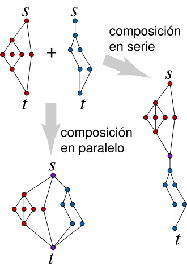
\includegraphics[width=0.8\linewidth]{images/image4.png}
\end{figure}
\textbf{Graf permutació bipartit} [3]
Un graf permutació és un graf tal que els seus vertex representen els elements d'una seqüència i les arestes representen parells d'elements revertits en una permutació concreta de la seqüència.[8]
